% This is sigproc-sp.tex -FILE FOR V2.6SP OF ACM_PROC_ARTICLE-SP.CLS
% OCTOBER 2002
%
% It is an example file showing how to use the 'acm_proc_article-sp.cls' V2.6SP
% LaTeX2e document class file for Conference Proceedings submissions.
% ----------------------------------------------------------------------------------------------------------------
% This .tex file (and associated .cls V2.6SP) *DOES NOT* produce:
%       1) The Permission Statement
%       2) The Conference (location) Info information
%       3) The Copyright Line with ACM data
%       4) Page numbering
%
%  However, both the CopyrightYear (default to 2002) and the ACM Copyright Data
% (default to X-XXXXX-XX-X/XX/XX) can still be over-ridden by whatever the author
% inserts into the source .tex file.
% e.g.
% \CopyrightYear{2003} will cause 2003 to appear in the copyright line.
% \crdata{0-12345-67-8/90/12} will cause 0-12345-67-8/90/12 to appear in the copyright line.
%
% ---------------------------------------------------------------------------------------------------------------
% It is an example which *does* use the .bib file (from which the .bbl file
% is produced).
% REMEMBER HOWEVER: After having produced the .bbl file,
% and prior to final submission,
% you need to 'insert'  your .bbl file into your source .tex file so as to provide
% ONE 'self-contained' source file.
%
% Questions regarding SIGS should be sent to
% Adrienne Griscti ---> griscti@acm.org
%
% Questions/suggestions regarding the guidelines, .tex and .cls files, etc. to
% Gerald Murray ---> murray@acm.org
%
% For tracking purposes - this is V2.6SP - OCTOBER 2002

\documentclass{acm_proc_article-sp-sigmod09}
\usepackage{url}
\usepackage{algorithm}
\usepackage[noend]{algpseudocode}
\usepackage{float}
\begin{document}
\algnewcommand\algorithmicforeach{\textbf{for each}}
\algdef{S}[FOR]{ForEach}[1]{\algorithmicforeach\ #1\ \algorithmicdo}
%
% --- Author Metadata here ---
\conferenceinfo{Data Mining}{Academic year 2018-2019}
%\setpagenumber{50}
%\CopyrightYear{2002} % Allows default copyright year (2002) to be over-ridden - IF NEED BE.
%\crdata{0-12345-67-8/90/01}  % Allows default copyright data (X-XXXXX-XX-X/XX/XX) to be over-ridden.
% --- End of Author Metadata ---

\title{Frequent itemset mining in tree-like sequences of complex objects \\ \large Nicol\`o Pomini [203319] and Marco Merlin[205263]}
%
% You need the command \numberofauthors to handle the "boxing"
% and alignment of the authors under the title, and to add
% a section for authors number 4 through n.

\numberofauthors{2}
%
\maketitle
\begin{abstract}
\dots
\end{abstract}

\terms{Data mining}

\keywords{Tree mining, frequent itemset mining}

\section{Introduction}
\dots

\section{Problem description}
How we understood the problem, and maybe the definition of pattern taken from the other report.

\section{General description}
General description of the idea and the differences with the other algorithms we know

\subsection{Assumptions}
\label{sec:assumptions}
For the sake of simplification, some assumption exists.

All the records contain at least four attributes: the \texttt{rid} to identify the record; the \texttt{tid} to recognize to which transaction the record belongs; a \texttt{parent} field, containing the \texttt{rid} of the parent record -- which can be empty in case the considered record is the root of a transaction; at least another attribute, which can have any name and any type. The latter kind of attribute is called \emph{generic attribute}. The patterns are built -- and consequently searched for -- on \emph{generic attributes}, and not on the other three types, which do not create any pattern since they are used to describe the structure of the transactions.

\newdef{definition}{Definition}
\begin{definition}
A \emph{generic attribute} is any attribute of a record which is not the \texttt{rid}, the \texttt{tid} or the \texttt{parent} attributes. These attributes represent the features of each record, and the patterns are made of \emph{generic attributes}.
\end{definition}

All the records are assumed to have the same attributes -- some of them may be empty. Each record has discrete values, belonging to finite sets of possible values. This assumption is needed to make the data mining project easier. From the point of view of the data generation, the absence of this constraint would not complicate anything.

\section{Problem statement}
A record $\boldsymbol{r}$ is a tuple, in the form $<a_1 \colon v_1, a_2 \colon v_2, \text{\dots}, a_n \colon v_n>$, where a pair $a_i \colon v_i$ represents an attribute-value relationship, where $a_i$ is the attribute and $v_i$ the value. These pairs can contain any kind of data, such as numbers or strings. To identify a record, is assumed that each one has an attribute called \emph{record id}, or \texttt{rid} for short.

A transaction $\boldsymbol{T}$ is a set of records $\{\boldsymbol{r_1}, \boldsymbol{r_2}, \text{\dots}, \boldsymbol{r_m}\}$ that forms a tree structure, which means that a transaction has a root record, which has some \emph{children records}, which in turn have some other children, and so on. To identify the transaction in which each record belongs, it is assumed that every record has an attribute called \emph{transaction id}, or \texttt{tid} for short.

\begin{figure}
\centering
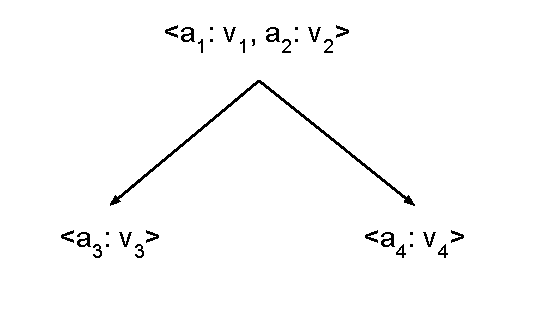
\epsfig{file=PatternExample.pdf}
\caption{An example of transaction, made of three records.}
\label{fig:transaction}
\end{figure}

Let us define a pattern.
\begin{definition}
A pattern is a set of ordered attributes and values belonging to possibly different records in the same transaction. In other words, a pattern is any ordered subset of $\bigcup\limits_{i=1}^{n} \bigcup\limits_{j=1}^{m} \boldsymbol{r_i}<a_j \colon v_j>$, where the ordering is given by the hierarchy of the transaction. For example, in Figure~\ref{fig:transaction} some possible example of pattern are $\{a_1 \colon v_1, a_3 \colon v_3\}$ or $\{a_2 \colon v_2, a_3 \colon v_3\}$, but not $\{a_4 \colon v_4, a_1 \colon v_1\}$, beacuse the latter breakes the hierarchic order.

A pattern has a tree structure, and it can be developed in three different ways.
\begin{itemize}
\item Horizontal -- which means that the pattern is made of a single record, with more than an attribute involved. This kind of pattern is a sort of a logical implication regarding two or more attributes in the same record, where the existence of a certain value implies the existence of some other values in the same record. Referring to Figure~\ref{fig:transaction}, the only possible horizontal pattern is $\{a_1 \colon v_1, a_2 \colon v_2\}$.
\item vertical -- when the pattern involves more than one record, and for each record one field is concerned, creating a tree structure. In this case, at least two records must be used to create such a pattern, otherwise any frequent value -- like every \texttt{tid} -- would be a pattern. The records in which appear a value belonging to the pattern do not have to be contiguous: in fact, it is possible to have a pattern made of three nodes -- for example $x, y, z$, with $x$ parent of $y$ and $y$ parent of $z$, where the existance of a value in $x$ implies the existance of a value in $z$, with any possible value in $y$. Referring to Figure~\ref{fig:transaction}, the possible vertical patterns are $\{a_1 \colon v_1, a_3 \colon v_3\}$, $\{a_2 \colon v_2, a_3 \colon v_3\}$, $\{a_1 \colon v_1, a_4 \colon v_4\}$, $\{a_2 \colon v_2, a_4 \colon v_4\}$, but also $\{a_3 \colon v_3, a_4 \colon v_4\}$. The latter is an example of a non-contiguos pattern: the parent has any value, and the two children have a value that implies the other one.
\item both horizontal and vertical -- the case of a vertical pattern, in which the records can have more than one attribute involved in the pattern. Referring to Figure~\ref{fig:transaction}, they can be $\{a_1 \colon v_1, a_2 \colon v_2, a_3 \colon v_3\}$, $\{a_1 \colon v_1, a_2 \colon v_2, a_4 \colon v_4\}$ or $\{a_1 \colon v_1, a_2 \colon v_2, a_3 \colon v_3, a_4 \colon v_4\}$.
\end{itemize}
\end{definition}

Given a set of transactions, the goal is to identify patterns of attributes that are frequent, which means transaction that appear at least a given number of time $f$.

\section{Algorithms}
\dots

\section{Experiments}
\dots

\section{Conclusions}
\dots

%\end{document}  % This is where a 'short' article might terminate
%
% The following two commands are all you need in the
% initial runs of your .tex file to
% produce the bibliography for the citations in your paper.
\bibliographystyle{abbrv}
\bibliography{sigproc}  % sigproc.bib is the name of the Bibliography in this case
% You must have a proper ".bib" file
%  and remember to run:
% latex bibtex latex latex
% to resolve all references
%
% ACM needs 'a single self-contained file'!
%
%APPENDICES are optional
%\balancecolumns
\appendix
%Appendix A
\section{Headings in Appendices}
The rules about hierarchical headings discussed above for
the body of the article are different in the appendices.
In the \textbf{appendix} environment, the command
\textbf{section} is used to
indicate the start of each Appendix, with alphabetic order
designation (i.e. the first is A, the second B, etc.) and
a title (if you include one).  So, if you need
hierarchical structure
\textit{within} an Appendix, start with \textbf{subsection} as the
highest level. Here is an outline of the body of this
document in Appendix-appropriate form:
\subsection{Introduction}
\subsection{The Body of the Paper}
\subsubsection{Type Changes and  Special Characters}
\subsubsection{Math Equations}
\paragraph{Inline (In-text) Equations}
\paragraph{Display Equations}
\subsubsection{Citations}
\subsubsection{Tables}
\subsubsection{Figures}
\subsubsection{Theorem-like Constructs}
\subsubsection*{A Caveat for the \TeX\ Expert}
\subsection{Conclusions}
\subsection{Acknowledgments}
\subsection{Additional Authors}
This section is inserted by \LaTeX; you do not insert it.
You just add the names and information in the
\texttt{{\char'134}additionalauthors} command at the start
of the document.
\subsection{References}
Generated by bibtex from your ~.bib file.  Run latex,
then bibtex, then latex twice (to resolve references)
to create the ~.bbl file.  Insert that ~.bbl file into
the .tex source file and comment out
the command \texttt{{\char'134}thebibliography}.
% This next section command marks the start of
% Appendix B, and does not continue the present hierarchy
\section{More Help for the Hardy}
The acm\_proc\_article-sp document class file itself is chock-full of succinct
and helpful comments.  If you consider yourself a moderately
experienced to expert user of \LaTeX, you may find reading
it useful but please remember not to change it.

% That's all folks!
\end{document}
